\documentclass{beamer}
\usetheme{Antibes}
\hypersetup{pdfpagemode=FullScreen}
\usepackage[italian]{babel}

\usepackage[backend = biber, citestyle = numeric]{biblatex}
\addbibresource{bibliografia/bibliografia.bib}

\title{Sulla sinergia tra apprendimento automatico e filtri di Bloom}
\author{{Giacomo Fumagalli}\\
{\and} \\
{Relatore: Prof. Dario Malchiodi} \\ {Correlatore: Prof. Marco Frasca}}
\date{}

\begin{document}

\frame{\titlepage}

\begin{frame}
\frametitle{Filtro di Bloom - Introduzione}
\begin{itemize}
    \item Un filtro di Bloom \cite{Bloom1970SpacetimeTI} è una struttura dati probabilistica, basata su funzioni di hash, spesso utilizzata per verificare l'appartenenza di un elemento a un dato insieme.
    \item Per definizione, un filtro di Bloom può generare solamente falsi positivi.
    \item Le operazioni che caratterizzano questa struttura dati sono inserimento e verifica dell'appartenenza di un elemento.
\end{itemize}
\end{frame}

\begin{frame}
\frametitle{Filtro di Bloom - Operazioni}
\centering
\begin{figure}[t!]
    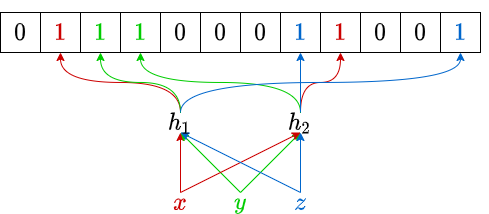
\includegraphics[height=\dimexpr0.4\textheight-0.5in]{immagini/3/bloomFilterInserimento.png}
    \caption{Esempio dell'operazione di inserimento.}
\end{figure}
\begin{figure}[t!]
    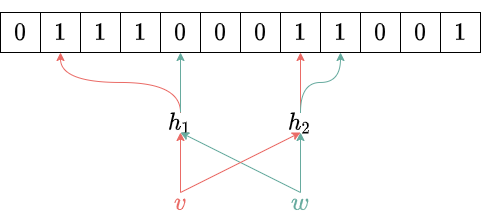
\includegraphics[height=\dimexpr0.4\textheight-0.5in]{immagini/3/bloomFilterCheck.png}
    \caption{Esempio dell'operazione di verifica dell'appartenenza.}
\end{figure}
\end{frame}

\begin{frame}{LBF e SLBF - Introduzione}
    \begin{itemize}
        \item Negli anni sono state sviluppate diverse varianti del filtro Bloom, al fine di aumentare ulteriormente l'efficienza della struttura originale. Esempi di queste varianti sono il filtro di Bloom appreso, o learned Bloom filter \cite{kraska2018case} (LBF), e il sandwiched learned Bloom filter \cite{10.5555/3326943.3326986} (SLBF).
        \item Sia LBF che SLBF si caratterizzano per l'utilizzo di un classificatore, al fine di ridurre lo spazio occupato dalla struttura.
        \item Un $\mathrm{LBF}(g, \tau, B)$ è caratterizzato da un classificatore $g$, una soglia $\tau$ e un filtro di Bloom $B$, chiamato filtro di backup.
        \item Un $\mathrm{SLBF}(B_0, g, \tau, B)$ è caratterizzato da un filtro di Bloom iniziale $B_0$, un classificatore $g$, una soglia $\tau$ e un filtro di backup $B$.
    \end{itemize}
\end{frame}

\begin{frame}
    \frametitle{LBF e SLBF - Controllo dell'appartenenza}
    \begin{figure}[htbp]
        \centering
        \begin{minipage}{0.30\textwidth}
        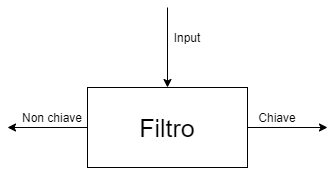
\includegraphics[width=\textwidth]{immagini/5_2/bloomFilter.png}
        \end{minipage}%%%
        \hfill
        \begin{minipage}{0.30\textwidth}
        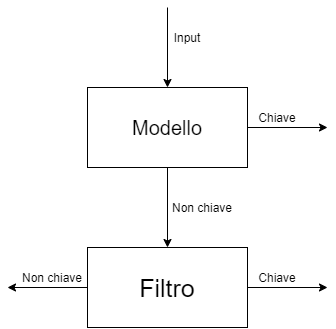
\includegraphics[width=\textwidth]{immagini/5_2/LBF.png}
        \end{minipage}
        \hfill
        \begin{minipage}{0.30\textwidth}
        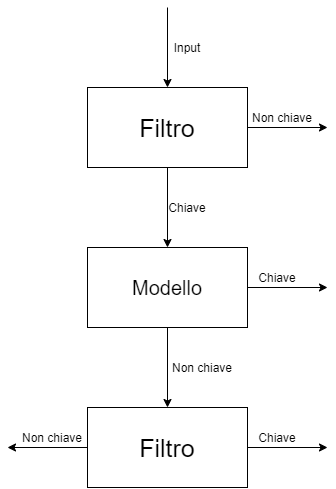
\includegraphics[width=\textwidth]{immagini/5_2/SLBF.png}
        \end{minipage}
    
        \begin{minipage}[t]{0.30\textwidth}
        \caption{Verifica dell'appartenenza in un filtro di Bloom.}
        \end{minipage}%%%
        \hfill
        \begin{minipage}[t]{0.30\textwidth}
        \caption{Verifica dell'appartenenza in un LBF.}
        \end{minipage}
        \hfill
        \begin{minipage}[t]{0.30\textwidth}
        \caption{Verifica dell'appartenenza in un SLBF.}
        \end{minipage}
    \end{figure}
\end{frame}

\begin{frame}
\frametitle{Esperimenti - Introduzione}
    \begin{itemize}
        \item Punto di partenza del tirocinio è l'articolo `An Empirical Analysis of the Learned Bloom Filter and its Extensions' \cite{ma2020}, l'obiettivo principale degli esperimenti effettuati è il confronto delle prestazioni dei filtri di Bloom appresi costruiti usando classificatori differenti da quelli dell'articolo.
        \item Il problema considerato è di classificazione di URL.
        \item Nello specifico, gli esperimenti effettuati si dividono in due categorie:
        \begin{itemize}
            \item esperimenti volti a misurare le performance dei classificatori nel problema considerato;
            \item esperimenti volti a confrontare le performance dei filtri di Bloom appresi costruiti utilizzando le due tipologie di classificatore.
        \end{itemize}
    \end{itemize}
\end{frame}

\begin{frame}
\frametitle{Esperimenti - Prestazioni dei classificatori}

\begin{itemize}
    \item Esperimenti volti a valutare le prestazioni dei classificatori nel problema di classificazione di URL.
    \item Si dividono in:
    \begin{itemize}
        \item Valutazione delle prestazioni della rete ricorrente:
        \begin{itemize}
            \item grandezza dell'insieme d'addestramento,
            \item sbilanciamento del dataset.
        \end{itemize}
        \item Valutazione delle prestazioni del percettrone: 
        \begin{itemize}
            \item selezione del modello.
        \end{itemize}
    \end{itemize}
    \item I risultati hanno evidenziato delle prestazioni migliori da parte del percettrone.
\end{itemize}
\end{frame}

\begin{frame}
    \frametitle{Esperimenti - Analisi dei filtri appresi}
    \begin{itemize}
        \item Esperimenti volti ad analizzare empiricamente i filtri di Bloom appresi costruiti usando le due tipologie di classificatore.
        \item Per entrambe le tipologie di filtro, vengono valutati:
        \begin{itemize}
            \item Tasso empirico di falsi positivi della struttura.
            \item Tasso di falsi negativi del classificatore.
            \item Taglia della struttura.
        \end{itemize} 
        \item Vengono valutati diversi valori per la soglia $\tau$ variando il rapporto $f_\tau/f$.
    \end{itemize}
\end{frame}

\begin{frame}
\frametitle{Risultati - Analisi empiriche LBF}
\begin{figure}[htbp]
    \centering
    \begin{minipage}{0.25\textwidth}
    \centering
    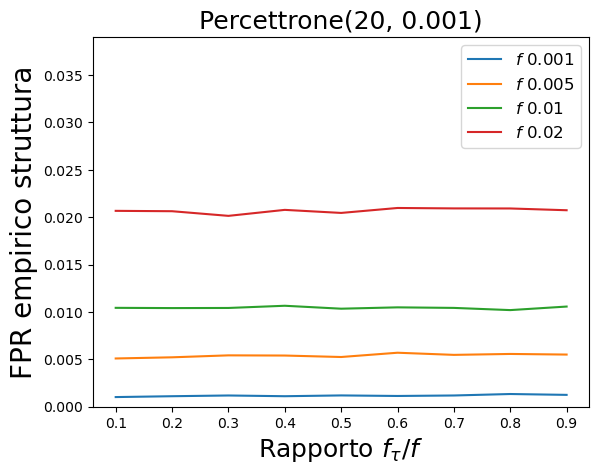
\includegraphics[width=\textwidth]{immagini/7/LBF/Percettrone(20, 0.001)_FPR.png}
    \end{minipage}%%%
    \hfill
    \begin{minipage}{0.25\textwidth}
    \centering
    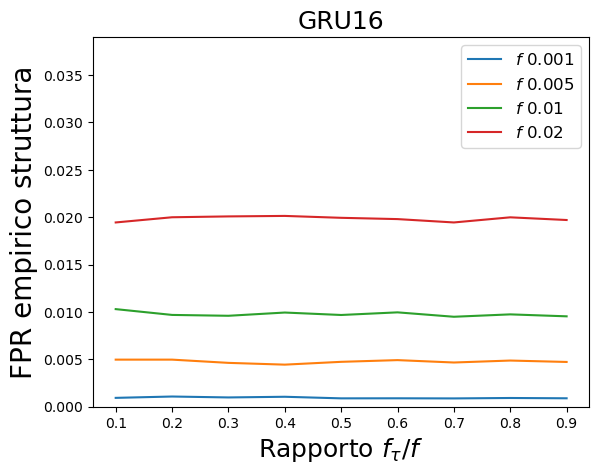
\includegraphics[width=\textwidth]{immagini/7/LBF/GRU16_FPR.png}
    \end{minipage}%%%
    \hfill
    \begin{minipage}{0.25\textwidth}
    \centering
    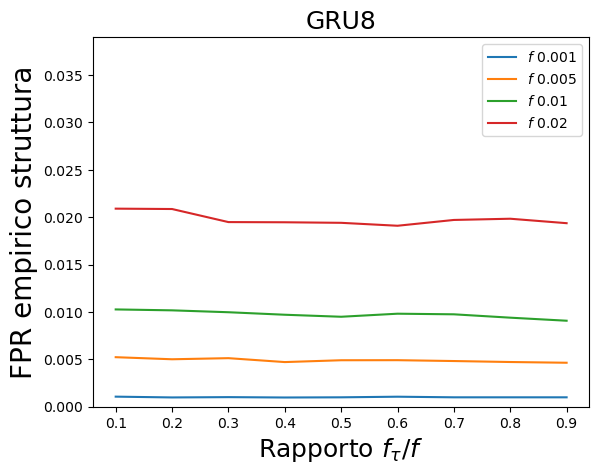
\includegraphics[width=\textwidth]{immagini/7/LBF/GRU8_FPR.png}
    \end{minipage}%%%
    \hfill
    \begin{minipage}{0.25\textwidth}
    \centering
    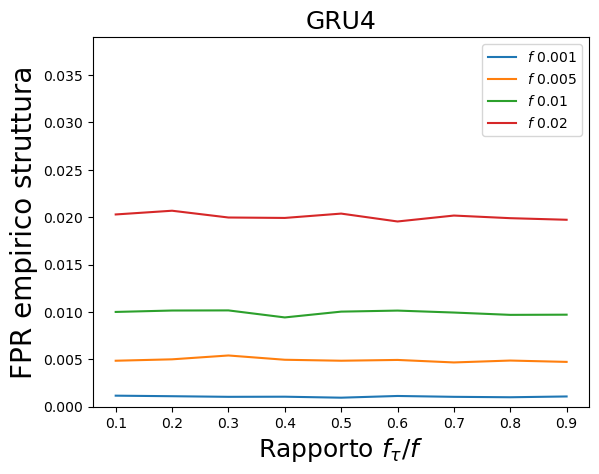
\includegraphics[width=\textwidth]{immagini/7/LBF/GRU4_FPR.png}
    \end{minipage}%%%
    \hfill

    \begin{minipage}[t]{\textwidth}
    \centering
    \caption{Tasso empirico di falsi positivi al variare di $\tau$}
    \end{minipage}%%%

    \centering
    \begin{minipage}{0.25\textwidth}
    \centering
    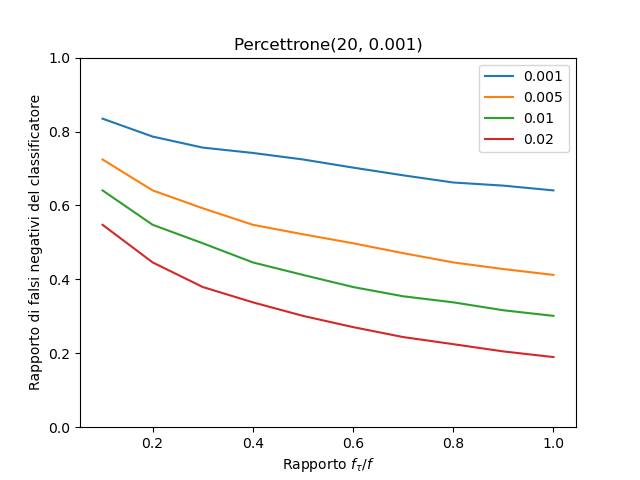
\includegraphics[width=\textwidth]{immagini/7/LBF/Percettrone(20, 0.001)_FNR.png}
    \end{minipage}%%%
    \hfill
    \begin{minipage}{0.25\textwidth}
    \centering
    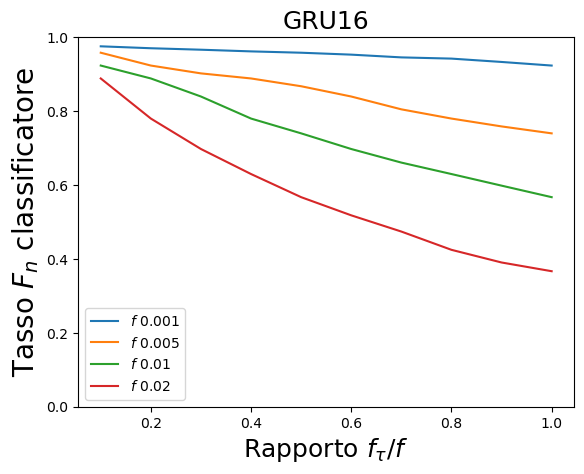
\includegraphics[width=\textwidth]{immagini/7/LBF/GRU16_FNR.png}
    \end{minipage}%%%
    \hfill
    \begin{minipage}{0.25\textwidth}
    \centering
    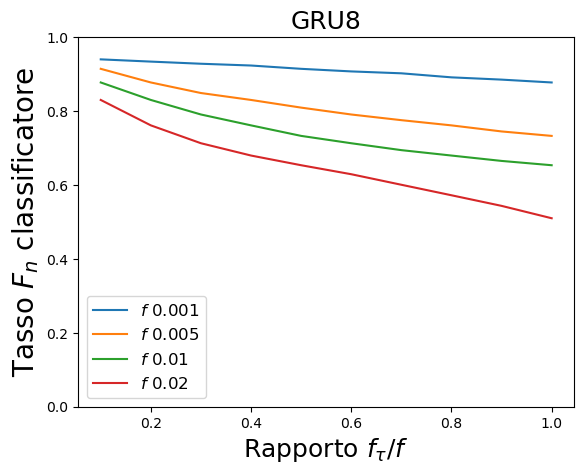
\includegraphics[width=\textwidth]{immagini/7/LBF/GRU8_FNR.png}
    \end{minipage}%%%
    \hfill
    \begin{minipage}{0.25\textwidth}
    \centering
    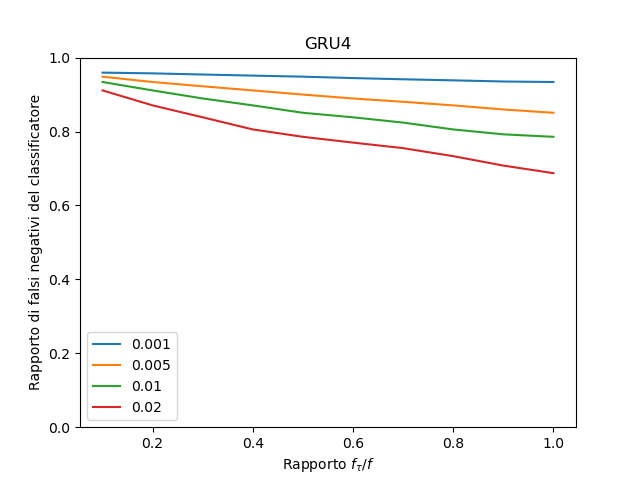
\includegraphics[width=\textwidth]{immagini/7/LBF/GRU4_FNR.png}
    \end{minipage}%%%
    \hfill

    \begin{minipage}[t]{\textwidth}
    \centering
    \caption{Tasso di falsi negativi al variare di $\tau$}
    \end{minipage}%%%
\end{figure}
\end{frame}

\begin{frame}
    \frametitle{Risultati - Analisi empiriche SLBF}
    \begin{figure}[htbp]
        \centering
        \begin{minipage}{0.25\textwidth}
        \centering
        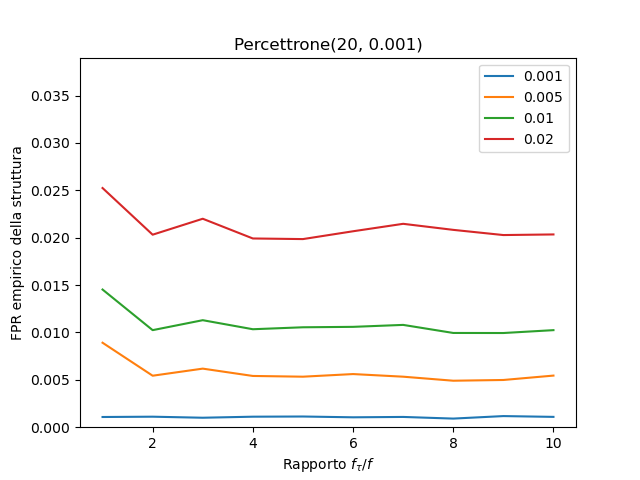
\includegraphics[width=\textwidth]{immagini/7/SLBF/Percettrone(20, 0.001)_FPR.png}
        \end{minipage}%%%
        \hfill
        \begin{minipage}{0.25\textwidth}
        \centering
        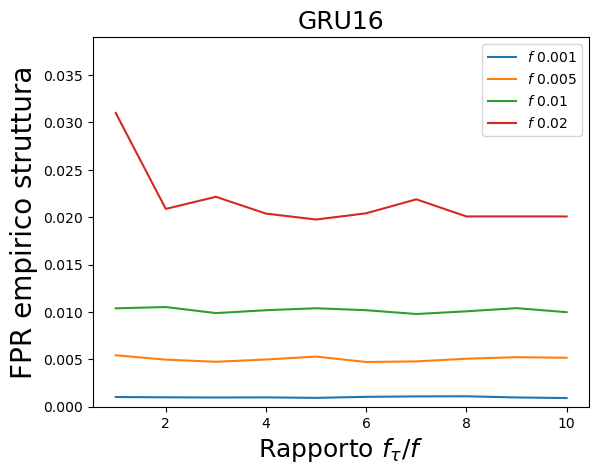
\includegraphics[width=\textwidth]{immagini/7/SLBF/GRU16_FPR.png}
        \end{minipage}%%%
        \hfill
        \begin{minipage}{0.25\textwidth}
        \centering
        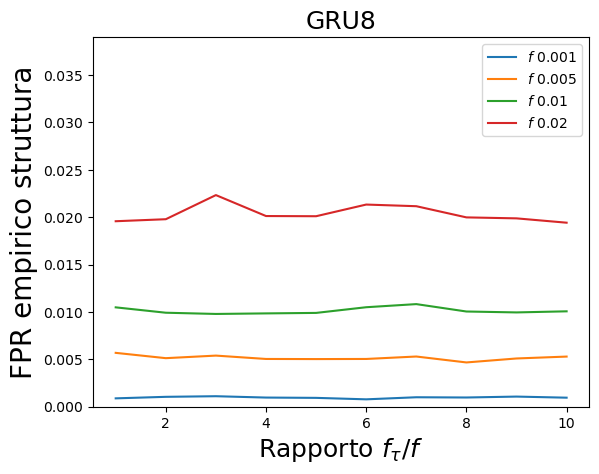
\includegraphics[width=\textwidth]{immagini/7/SLBF/GRU8_FPR.png}
        \end{minipage}%%%
        \hfill
        \begin{minipage}{0.25\textwidth}
        \centering
        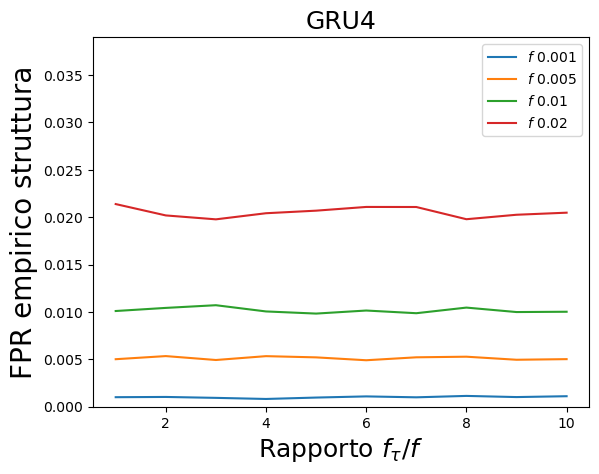
\includegraphics[width=\textwidth]{immagini/7/SLBF/GRU4_FPR.png}
        \end{minipage}%%%
        \hfill
    
        \begin{minipage}[t]{\textwidth}
        \centering
        \caption{Tasso empirico di falsi positivi al variare di $\tau$.}
        \end{minipage}%%%
    
        \centering
        \begin{minipage}{0.25\textwidth}
        \centering
        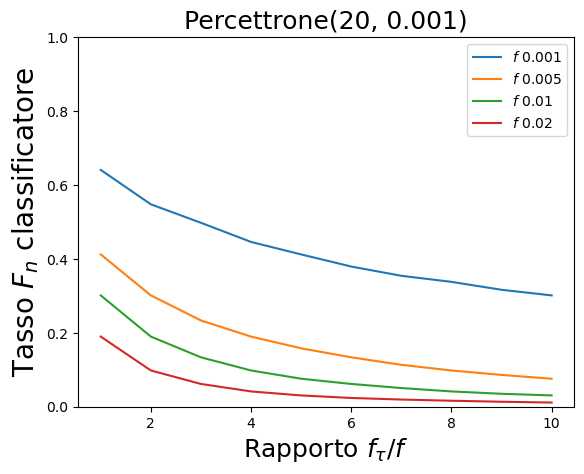
\includegraphics[width=\textwidth]{immagini/7/SLBF/Percettrone(20, 0.001)_FNR.png}
        \end{minipage}%%%
        \hfill
        \begin{minipage}{0.25\textwidth}
        \centering
        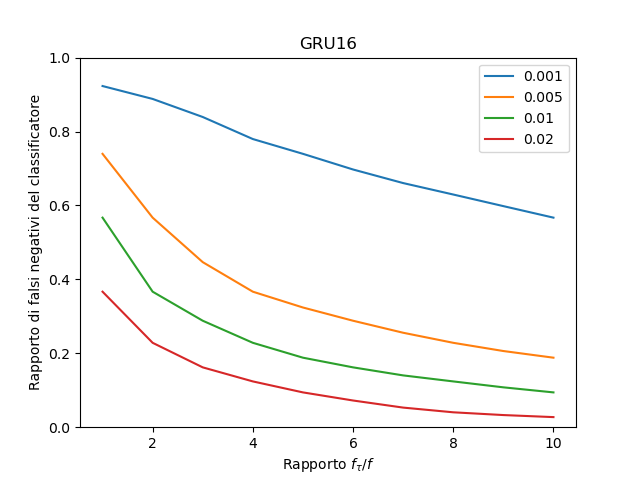
\includegraphics[width=\textwidth]{immagini/7/SLBF/GRU16_FNR.png}
        \end{minipage}%%%
        \hfill
        \begin{minipage}{0.25\textwidth}
        \centering
        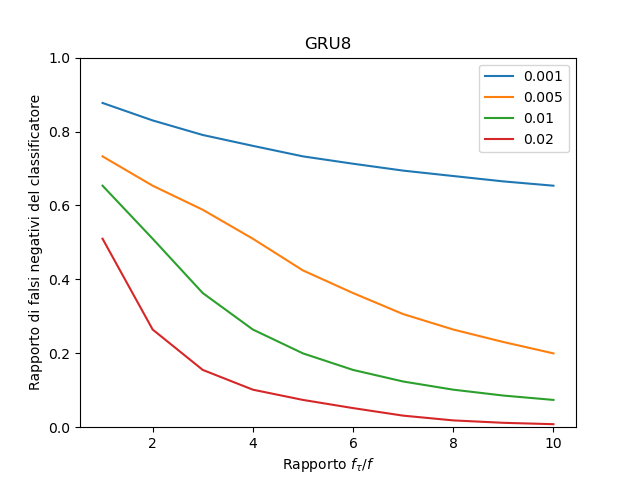
\includegraphics[width=\textwidth]{immagini/7/SLBF/GRU8_FNR.png}
        \end{minipage}%%%
        \hfill
        \begin{minipage}{0.25\textwidth}
        \centering
        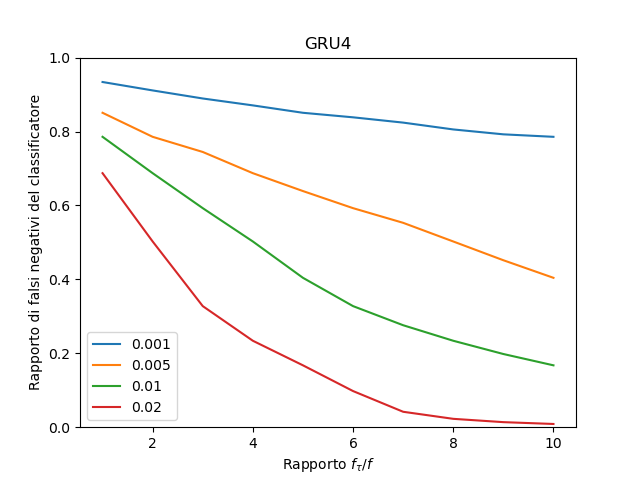
\includegraphics[width=\textwidth]{immagini/7/SLBF/GRU4_FNR.png}
        \end{minipage}%%%
        \hfill
    
        \begin{minipage}[t]{\textwidth}
        \centering
        \caption{Tasso di falsi negativi al variare di $\tau$.}
        \end{minipage}%%%
    \end{figure}
    \end{frame}

\begin{frame}
    \frametitle{Risultati - Spazio occupato}
    \begin{figure}[htbp]
        \centering

        \begin{minipage}{0.25\textwidth}
        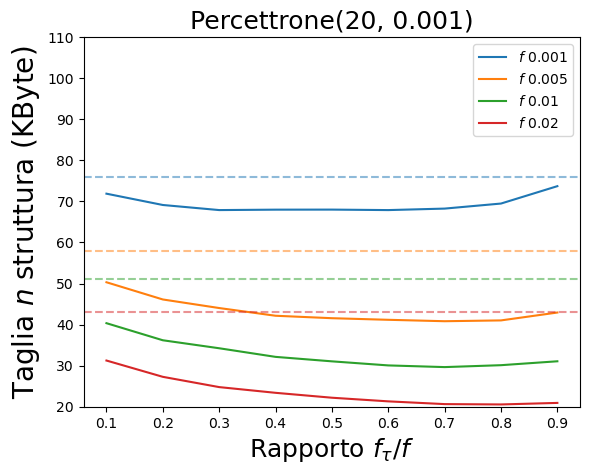
\includegraphics[width=\textwidth]{immagini/7/LBF/Percettrone(20, 0.001)_Taglia.png}
        \end{minipage}%%%
        \hfill
        \begin{minipage}{0.25\textwidth}
        \centering
        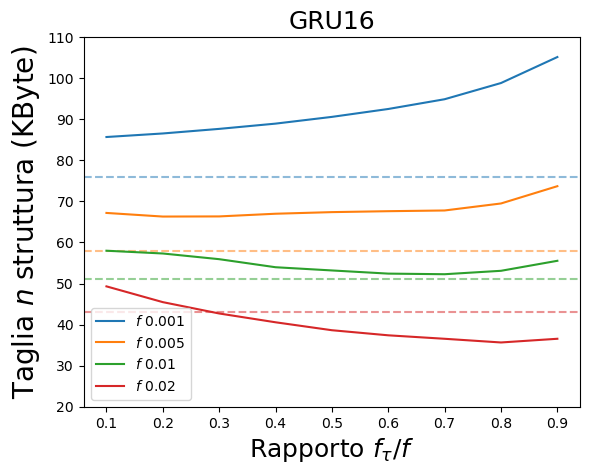
\includegraphics[width=\textwidth]{immagini/7/LBF/GRU16_Taglia.png}
        \end{minipage}%%%
        \hfill
        \begin{minipage}{0.25\textwidth}
        \centering
        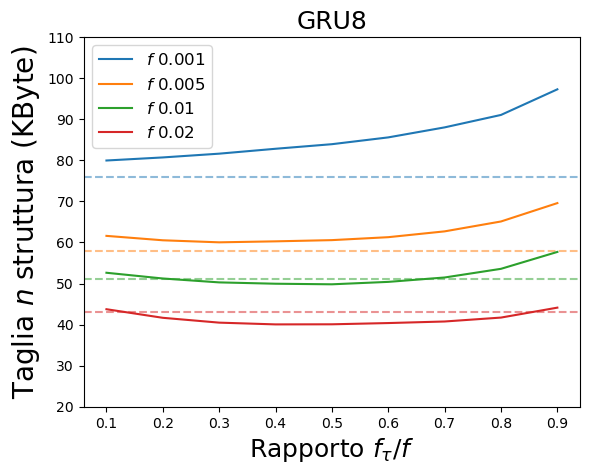
\includegraphics[width=\textwidth]{immagini/7/LBF/GRU8_Taglia.png}
        \end{minipage}%%%
        \hfill
        \begin{minipage}{0.25\textwidth}
        \centering
        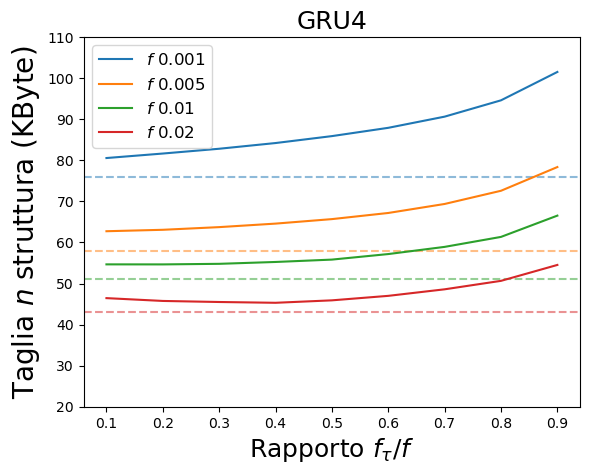
\includegraphics[width=\textwidth]{immagini/7/LBF/GRU4_Taglia.png}
        \end{minipage}%%%
        \hfill

        \begin{minipage}[t]{\textwidth}
        \centering
        \caption{Spazio occupato dai LBF al variare di $\tau$.}
        \end{minipage}%%%
    

        \begin{minipage}{0.25\textwidth}
        \centering
        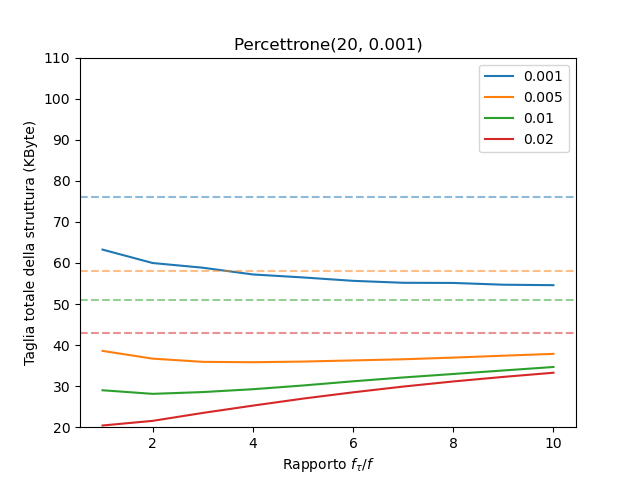
\includegraphics[width=\textwidth]{immagini/7/SLBF/Percettrone(20, 0.001)_Taglia.png}
        \end{minipage}%%%
        \hfill
        \begin{minipage}{0.25\textwidth}
        \centering
        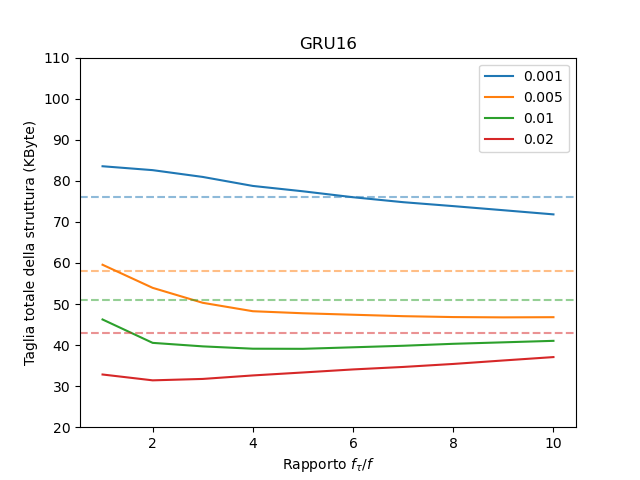
\includegraphics[width=\textwidth]{immagini/7/SLBF/GRU16_Taglia.png}
        \end{minipage}%%%
        \hfill
        \begin{minipage}{0.25\textwidth}
        \centering
        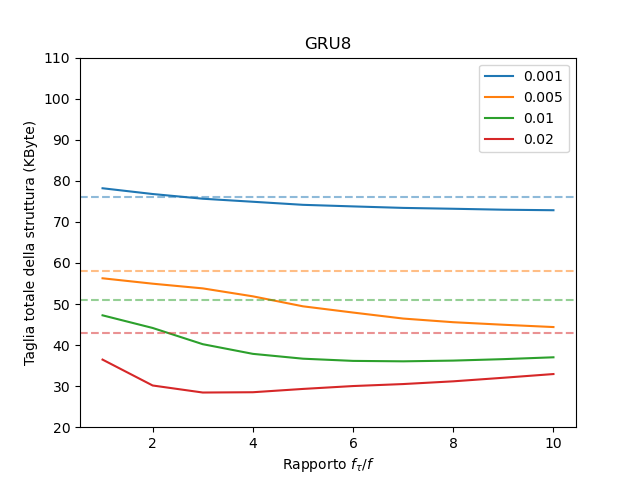
\includegraphics[width=\textwidth]{immagini/7/SLBF/GRU8_Taglia.png}
        \end{minipage}%%%
        \hfill
        \begin{minipage}{0.25\textwidth}
        \centering
        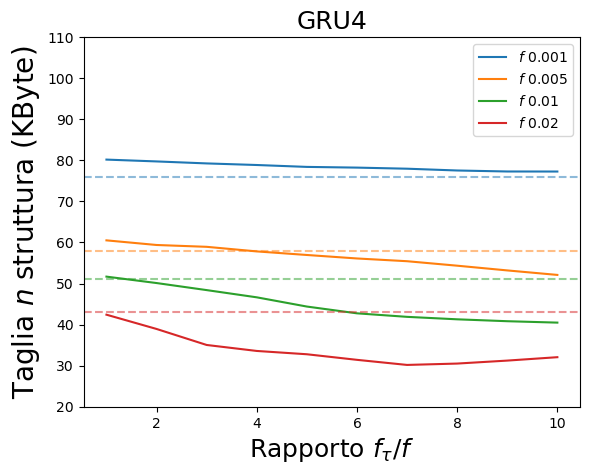
\includegraphics[width=\textwidth]{immagini/7/SLBF/GRU4_Taglia.png}
        \end{minipage}%%%
        \hfill

        \begin{minipage}[t]{\textwidth}
        \centering
        \caption{Spazio occupato dai SLBF al variare di $\tau$.}
        \end{minipage}%%%
    \end{figure}
\end{frame}

\begin{frame}
\frametitle{Risultati - Confronto tra LBF e SLBF}
\begin{figure}[htbp]
    \centering
    \begin{minipage}{0.50\textwidth}
    \centering
    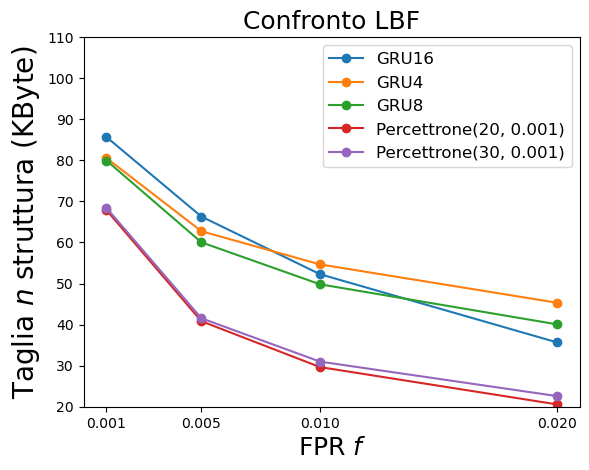
\includegraphics[width=\textwidth]{immagini/7/LBF/Confronto.png}
    \end{minipage}%%%
    \hfill
    \begin{minipage}{0.50\textwidth}
    \centering
    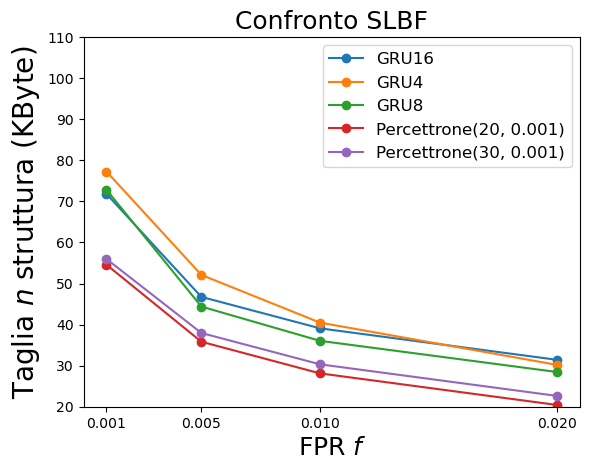
\includegraphics[width=\textwidth]{immagini/7/SLBF/Confronto.png}
    \end{minipage}%%%
\end{figure}
\end{frame}

\begin{frame}[allowframebreaks]
\frametitle{Bibliografia}
\printbibliography
\end{frame}
\end{document}